\documentclass[
    oneside,
    a4paper,
    12pt
]{book}
\usepackage[
    paperwidth=21cm,
    paperheight=29cm,
    vmargin={2.5cm},
    left={3.0cm},
    right={2.5cm},
    centering,
    pdftex
]{geometry}
\usepackage[brazilian]{babel}
\usepackage{times}
\usepackage{lettrine}
\usepackage{graphics,graphicx}
\usepackage{lscape, setspace}
\usepackage{subfigure}
\usepackage[latin1]{inputenc}
\usepackage{natbib}
\bibpunct{(}{)}{;}{a}{,}{;}

%*** BASIC INFORMATION ***%
\newcommand{\university}{Universidade Federal de Minas Gerais}
\newcommand{\institution}{Instituto de Geociências}
\newcommand{\department}{Departamento de Geografia}
\newcommand{\documentTitle}{Título da tese}
\newcommand{\documentAuthor}{Luiz Felipe Matos Pedone}
\newcommand{\documentAdvisor}{Dr. Philippe Maillard}
\newcommand{\documentYear}{2017}

\begin{document}
\onehalfspace
\frontmatter
\pagestyle{empty}
\title{
    \large
    {\university}\\
    {\institution}\\
    {\department}\\
    \vspace{2in}\huge\textbf{\documentTitle}\vspace{1.0in}
}
\author{\hspace{3in}\large \documentAuthor\vspace{0.7in}}
\date{Belo Horizonte\\{\documentYear}}

\maketitle
\begin{centering}
\large {\documentAuthor}\\
\vspace{2in}
\huge\textbf{\documentTitle}\\
\vspace{1in}
\normalsize
\raggedleft\parbox{8cm}{\raggedright{Tese apresentada ao Programa de Graduação do {\department} da {\university}, como requisito parcial à obtenção do título de licenciado em Geografia.\\
\vspace{0.5in}
Orientador: }{\documentAdvisor}}\\
\vspace{1in}
\centering \large Belo Horizonte\\{\documentYear}\\
\normalsize
\newpage
\raggedright{Tese defendida e aprovada, em 06 de julho de 2006, pela Banca Examinadora constituída pelos doutores e professores:}\\
\centering
\vspace{1.5in}

\begin{center}\begin{tabular}{c c c c c}
  \hline
   & & Membro  Banca 1 &  & \\
   \vspace{1 in}\\
  \hline
   & & Membro  Banca 2 &  & \\
   \vspace{1 in}\\
  \hline
   & & Membro  Banca 3 &  & \\
   \vspace{1 in}\\
  \hline
   & & Membro  Banca 4 &  & \\
   \vspace{1 in}\\
  \hline
   & & Prof. {\documentAdvisor} &  & \\

\end{tabular}\end{center}

\end{centering}

\tableofcontents

\listoffigures

\listoftables
\pagestyle{plain}
\frontmatter

\chapter{Resumo} Meu resumo.

\chapter{Agradecimentos} Aos deuses

\chapter{Siglas e Símbolos} SIGLAS
\begin{itemize}
    \item 5s: Simulation of the Satellite Signal in the Solar Spectrum
    \item ASC: Agence Spatialle Canadienne
    \item ANOVA: Análise de Variância
    \item AVHRR: Advanced Very High Resolution Radiometer
    \item CAP: Circunferência a Altura do Peito
    \item CBERS: China-Brazil Earth Resources Satellite
    \item CCD: Couple Charged Device
    \item DAP: Diâmetro a Altura do Peito
    \item DR: Densidade Relativa
    \item DT: Densidade de árvores no transecto
    \item EMBRAPA: Empresa Brasileira de Pesquisa Agropecuária
    \item ETM+: Enhanced Thematic Mapper Plus
    \item GLA: Gap Light Analyser
    \item GPS: Global Positioning System
    \item HH: Horizontal-Horizontal
    \item IAF: Índice de Área Foliar
    \item IBAMA: Instituto Brasileiro do Meio Ambiente e dos Recursos Renováveis
    \item IEF-MG: Instituto Estadual de Florestas de Minas Gerais
    \item INPE: Instituto Nacional de Pesquisas Espaciais
    \item IS: Índice de Shannon
    \item JANASA: Januária Agropecuária S.A.
    \item LUT: Look up Table
    \item LUT: Look up Table
    \item MDE: Modelo Digital de Elevação
    \item MDM: Minimum Distance to Mean
    \item ML: Maximum Likelihood
    \item MODIS: Moderate Resolution Imaging Spectroradiometer
    \item MSS: Multi-Spectral Scanner
    \item ND: Número Digital
    \item NDVI: Normalized Difference Vegetation Index
    \item NDVI$_{A}$: Imagem de NDVI do mês de agosto
    \item NDVI$_{M}$: Imagem de NDVI do mês de maio
    \item PAD: Porcentagem de Abertura do Dossel
    \item PARNA: Parque Nacional
    \item PEVP: Parque Estadual Veredas do Peruaçu
    \item RADAR: Radio Detection and Ranging
    \item RAR: Radar de Abertura Real
    \item RIXacriabá: Reserva Indígena Xacriabá
    \item Ruralminas: Fundação Rural de Minas Gerais
    \item S2$_{A}$: Imagem RADARSAT S2 do mês de abril
    \item S2$_{S}$: Imagem RADARSAT S2 do mês de setembro
    \item S6$_{A}$: Imagem RADARSAT S6 do mês de abril
    \item S6$_{S}$: Imagem RADARSAT S2 do mês de setembro
    \item SAM: Spectral Angle Mappe
    \item SAR: Synthetic Aperture Radar
    \item SGE: Serviço Geográfico do Exército
    \item SGE: Serviço Geográfico do Exército
    \item SPOT: Systeme Pour l'Observation de la Terre
    \item SSC: Spectral-spatial Classifier
    \item SUDENE: Superintendência de Desenvolvimento do Nordeste
    \item TM: Thematic Mapper
    \item UFMG: Universidade Federal de Minas Gerais
    \item UFV: Universidade Federal de Viçosa
    \item UG: Umidade Gravimétrica
    \item VV: Vertical-Vertical
\end{itemize}

SÍMBOLOS
\begin{itemize}
    \item ß°: Brilho do radar
    \item {$\sigma$}º: Coeficiente de retroespalhamento do radar
    \item $\sigma$: Desvio padrão
    \item $\lambda$: Comprimento de onda
    \item $\mu$: Média
%    \item $\mi$m: Micrômetro
    \item {$\rho$}: Reflectância aparente no topo da atmosfera

\end{itemize}

\mainmatter    %********************** a numeração árabe começa aqui *********************
\chapter{INTRODUÇÃO}\lettrine{O}{cerrado}, ou savana brasileira, é uma forma de vegetação complexa, bla bla bla...

O principal objetivo deste trabalho consiste em,  bla bla bla... para permitir: 1) fazer isso; e 2) aquilo.

Foram formulados cinco objetivos específicos a fim  bla bla bla...:
\begin{enumerate}
    \item reconstruir a história da área de estudo  bla bla bla...;
    \item buscar um maior entendimento acerca  bla bla bla...;
    \item identificar as propriedades preponderantes  bla bla bla...;
    \item caracterizar a resposta em dados  bla bla bla...;
    \item propor modelos estatísticos para  bla bla bla....
\end{enumerate}

A pesquisa deve ser desenvolvida em uma área na qual as mudanças de uso da terra sejam conhecidas,  bla bla bla....

O trabalho foi dividido em cinco capítulos. O presente capítulo que introduz o assunto e traz os objetivos da pesquisa. O Capítulo 2 que apresenta as características ambientais e históricas da área de estudo. O Capítulo 3 traz uma fundamentação teórica sobre os principais temas que circundam esta pesquisa. O Capítulo 4 expõe as etapas metodológicas envolvidas no desenvolvimento do trabalho. O Capítulo 5 que apresenta e discute os resultados encontrados. E por fim o Capítulo 6 sintetiza os resultados do trabalho e traz algumas considerações.

\chapter{ÁREA DE ESTUDO}

\lettrine{A}{área} de estudo bla bla bla....  A figura \ref{fig:estudo}.

O \cite{ATeuner95} é um cara legal.

\begin{figure}[bp]
 \begin{center}
\fbox{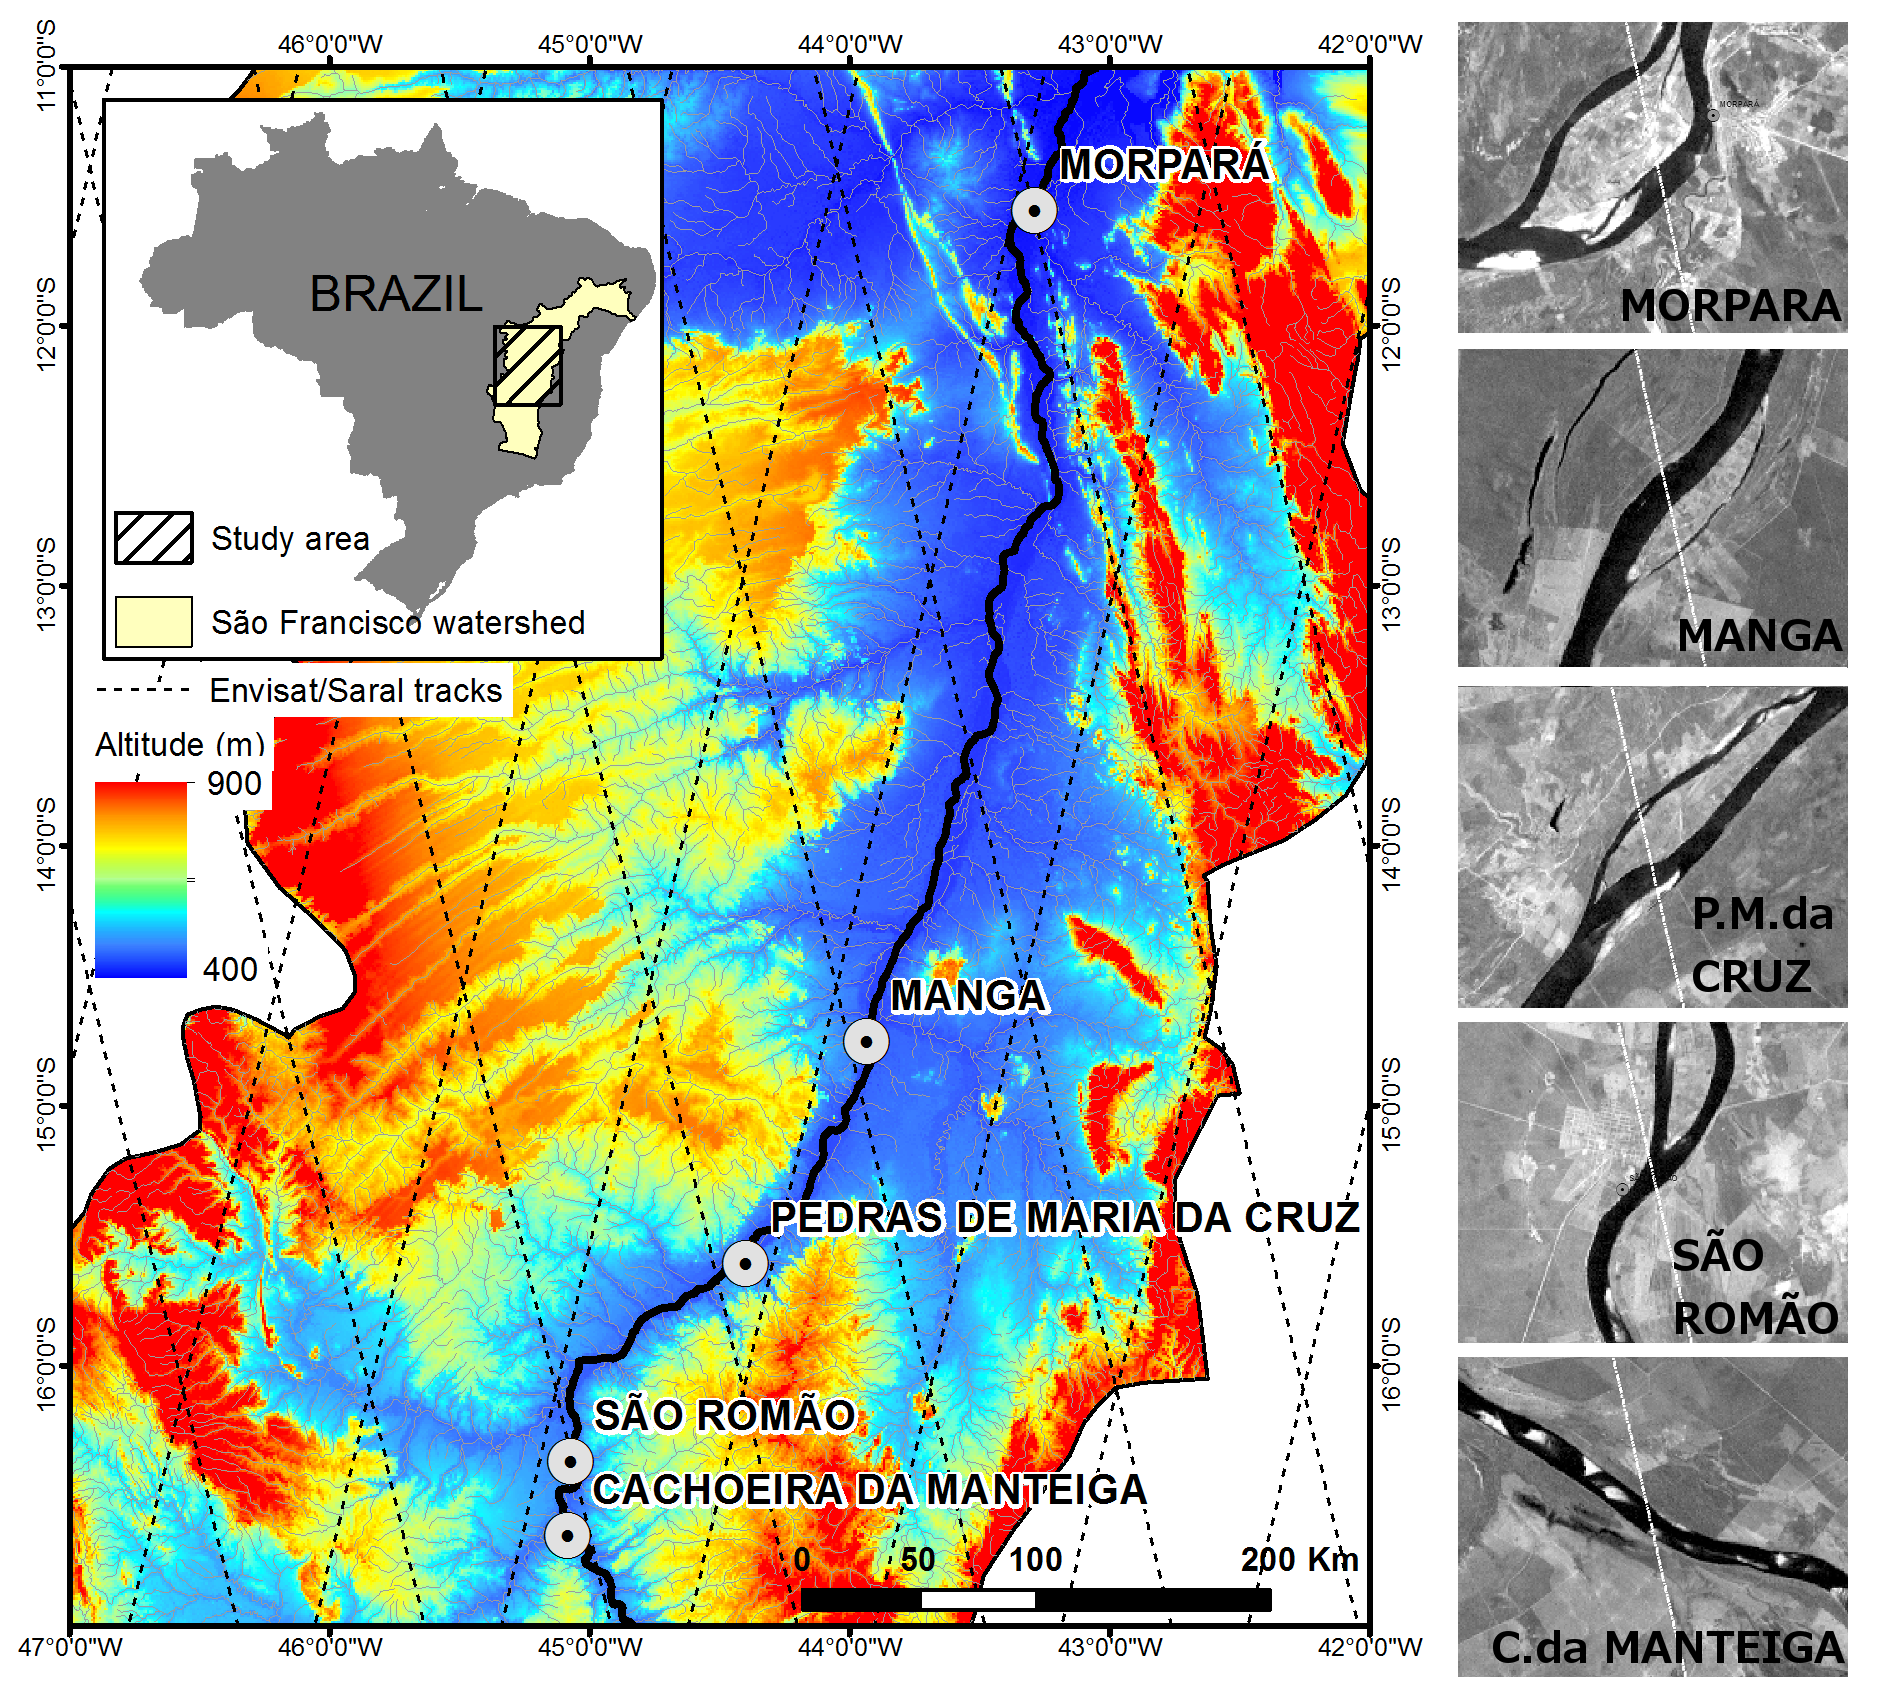
\includegraphics[width=0.35\columnwidth]{figuras/Localization_SF.png}}
\end{center}
\caption{ \label{fig:estudo} Mapa de localização ....}
\end{figure}

\begin{table}[h]
  \centering
  \caption{$r^{2}$ para os modelos testados.}\label{TB:regressao}
\begin{tabular}{c c c c c}
  \hline
  Parameter & All & S2A,S & S2A+S6A & S2A+S6S \\
  \hline
  DBH & 17 & 11 & - & - \\
  LAI & 16 & 10 & - & - \\
  SI & 16 & 15 & - & - \\
  TD & \textbf{25} & \emph{24} & \emph{21} & \emph{22} \\
  GM & \textbf{89} & \emph{50} & \emph{54} & \emph{60} \\
  \hline
  \multicolumn{5}{l}{All = all four images, S2A = S2 Abril, S2S = S2 September,}\\
  \multicolumn{5}{l}{S6A = S6 Abril, S6S = S6 September,.}
\end{tabular}
\end{table}


\chapter{CONSIDERAÇÕES FINAIS} \lettrine{B}{la} bla bla...


\bibliography{References_PM}
\bibliographystyle{chicago_pt2}

\appendix

\end{document}
